\chapter{Solutions for Burgers' Equation in the Deterministic Version}
\label{Chapter_3} 
	
	This chapter is one of the most important, since we will begin with the development of the main objective of this work. We will construct two spectral methods known as Fourier-Galerkin and Fourier-Collocation using the projection and interpolation operators respectively, considering an initial value problem that will be defined using our objective equation presented in (\ref{Burgers_Equation}). \\
	
	For this, to illustrate what we have studied in the Chapter (\ref{Chapter_2}), we will consider the function space $H^q_p [0, 2 \pi]$ with the norm defined in (\ref{sobolev_norm}) for some $q$ that will be specified later. We will assume that the problems have solutions $u(x, t) \in H^q_p [\mathcal{D}]$ for every $t \in I$, where $\mathcal{D} = [x_L, x_R]$ for some fixed reals $ x_L $, $ x_R $ and $I = [0, T]$ with $T> 0$. So, given some real $\alpha \geq 0$ and an initial condition function $u_0 (x) \in H^q_p [\mathcal{D}]$, our initial value problem is as follows
	\begin{align}
	\label{IVP_Burgers}
		\left \lbrace \begin{array}{ll}
			\frac{\partial u}{\partial t} + \frac{1}{2} (u^2)_x = \alpha \frac{\partial^2 u}{\partial x}, \hspace{2mm} 0 < t \leq T, \hspace{2mm} x \in I \\
			\\
			u(x, 0) = u_0(x), \hspace{2mm} x \in I
		\end{array}  \right .
	\end{align}
	
	The analytical solution of the previous problem was given in (\ref{Exact_Solution}), and we observe that it is not easy to evaluate it directly. Therefore, it is necessary to choose a suitable method of numerical integration to calculate the integrals involved, since they have exponential behavior that is noticeably affected when the parameter $\alpha$ is very small. However, precision problems can also arise because arithmetic operations can generate considerable errors if they are not performed correctly, and therefore this equation is not a good choice for finding solutions to the problem. \\
	
	In the next section, we will present the aforementioned spectral methods considering the linear problem obtained by using the transformation given by (\ref{Hopf_tranform}), And this will allow us to approximate the solutions of the problem (\ref{IVP_Burgers}) More easily and with excellent precision. In addition, this will give us the advantage of having solutions that can be considered exact and use them to compare them with those that will be obtained in the numerical experiments that we will describe in the second section when implementing these methods for the nonlinear problem (\ref{IVP_Burgers}), Since we will observe that the precision will be much less because we will need to use numerical methods to solve in the variable $t$, decreasing with respect to the parameter $\alpha$.
    
	\section{Fourier Spectral Methods}
	
	In the following sections we will work with the problem obtained by the transformation of the problem (\ref{Hopf_tranform}) given by
	\begin{align}
		u(x, t) = - 2 \alpha \frac{\partial_{x} \varphi(x, t)}{\varphi(x, t)} = - 2 \alpha \left( \log{\varphi(x, t)} \right)_x
	\end{align}
	with $\alpha > 0$, and $\varphi$ solves the following initial value problem
	\begin{align}
	\label{Bugers_Lineal}	
		\left \lbrace \begin{array}{ll}
			\frac{\partial \varphi}{\partial t} = \alpha \varphi_{xx}, \hspace{2mm} 0 < t \leq T, \hspace{2mm} x \in I \\
			\\
			\varphi(x, 0) = \displaystyle \varphi_0 (x) = e^{- \int_{0}^{x} \frac{u_0(y)}{2 \alpha} dy}, \hspace{2mm} x \in I
		\end{array}  \right .
	\end{align}
	\subsection{Fourier-Galerkin}
    \label{Galerkin}
	\vspace{0.3cm} 
	
	
	In chapter \ref{Chapter_2} we saw that for a function $\varphi \in H^2_p [0, 2 \pi]$ it can be written as
	\begin{align}
	\label{Expansion_phi}	
		\varphi (x, t) = \displaystyle \sum_{|n| \leq \infty} \hat{\varphi}_n (t) \phi_n (x), \hspace{2mm} \hat{\varphi}_n (t) = \frac{1}{2 \pi} \left\langle \varphi (x, t), \phi_n (x) \right\rangle  
	\end{align}
	where $\phi_n (x) = e^{inx}$, and let's assume that this function is the solution of the problem (\ref{Bugers_Lineal}).\\
	
	The Fourier-Galerkin method will be constructed using the project operator described in (\ref{proyection_operator}) to project and force the function $\varphi$ to satisfy the problem (\ref{Bugers_Lineal}) on a space that will be defined a continuation. \\
	
	Let $V_N$ the space of trigonometric polynomials of degree $2N + 1$ given by $V_N = B_N \cap H^2_p [0, 2 \pi]$, where $B_N = span\{\phi_n (x) : |n| \leq N\}$. Then for $\varphi \in V_N$ we can obtain its expansion as  
	\begin{align}
	\label{Expansion_phi_N}	
		\varphi_N (x, t) = \displaystyle \sum_{|n| \leq N} \hat{\varphi}_n (t) \phi_n (x), \hspace{2mm} \hat{\varphi}_n (t) = \frac{1}{2 \pi} \left\langle \varphi (x, t), \phi_n (x) \right\rangle  
	\end{align} 
	
	Substituting (\ref{Expansion_phi}), and (\ref{Expansion_phi_N}) into the equation (\ref{Bugers_Lineal}) to taking the difference as follows
	\begin{align*}
		\left[ \frac{\partial}{\partial t} \varphi_N - \alpha \frac{\partial^2}{\partial x} \varphi_N \right] - \left[ \frac{\partial \varphi}{\partial t} - \alpha \frac{\partial^2 \varphi}{\partial x} \right] = R_N (x, t)   
	\end{align*}
	where $R_N (x, t)$ is a residual function, and since the second term is exactly zero because $\varphi$ is the exact solution we have to
	\begin{align*}
		\frac{\partial}{\partial t} \varphi_N -  \alpha \frac{\partial^2}{\partial x} \varphi_N = R_N (x, t)
	\end{align*}
	
	In the Fourier-Galerkin method, it is desired that the remainder $R_N$ belong to the orthogonal space of $ V_N $, that is, for every $\varphi, \phi \in V_N $ such that $\langle \varphi - \mathcal{P}_N \varphi, \phi \rangle = 0$. This is achieved by forcing for each $|n| \leq N$ the following condition
	\begin{align}
		\left\langle R_N, \phi_n \right\rangle = \left\langle \frac{\partial \varphi_N}{\partial t} - \alpha \frac{\partial^2 \varphi_N}{\partial x^2}, \phi_n \right\rangle = 0, \hspace{2mm}  \hspace{2mm} \phi_n \in V_N, \hspace{2mm} \forall t > 0
	\end{align}
	or equivalently
	\begin{align*}
		\displaystyle \int_{\mathcal{D}} \frac{\partial}{\partial t} \varphi_N (x, t) \overline{\phi_n (x)} dx = \alpha \int_{\mathcal{D}} \frac{\partial^2}{\partial x^2} \varphi_N (x, t) \overline{\phi_n (x)} dx , \hspace{2mm}  \hspace{2mm} \phi_n \in V_N, \hspace{2mm} \forall t > 0
	\end{align*}
	
	\noindent Using the orthogonality $\langle \phi_k, \phi_n \rangle = 2 \pi \delta_{kn}$, for each $n$ fixed we have to
	\begin{align*}
		\left\langle \frac{\partial \varphi_N}{\partial t}, \phi_n  \right\rangle = \left\langle \displaystyle \sum_{ |k| \leq N} \frac{d \hat{\varphi}_k (t)}{dt} \phi_k, \phi_n  \right\rangle = 2 \pi \frac{d \hat{\varphi}_n (t)}{dt}
	\end{align*}
	
	Note that the spatial interval is not the desired one, for this we are going to define the following linear transformation from $\mathcal{D}_p = [0, 2 \pi]$ to $\mathcal{D} = [x_L, x_R]$ given by $x = P z + x_L$ to escalate the problem, where $P = \frac{x_R - x_L}{2 \pi}$ and $z \in \mathcal{D}_p$. Then, using the chain rule we can rewritten the derivatives as
	\begin{align*}
		\frac{\partial^2 \varphi_N}{\partial x^2} = P^2 \frac{\partial^2 \varphi_N}{\partial x^2} 
	\end{align*}
	and using $\frac{\partial^2}{\partial x^2} \phi_n (x) = -P^2 n^2 \phi_n (x)$ we have to  
	\begin{align*}
		\alpha \left\langle \frac{\partial^2 \varphi_N}{\partial x^2}, \phi_n \right\rangle = -2 \pi \alpha P^2 n^2 \hat{\varphi}_n (t), \hspace{2mm} |n| \leq N
	\end{align*}
	
	\noindent Therefore, we have the next ODE
	\begin{align*}
		\frac{d \hat{\varphi}_n (t)}{dt} = - \alpha P^2 n^2 \hat{\varphi}_n (t), \hspace{2mm} |n| \leq N 
	\end{align*}
	which is solved using the projection of the initial condition given by
	\begin{align}
	\label{Galerkin_Linear}	
		\varphi_N (x, 0) = \displaystyle \sum_{|n| \leq N} \hat{\varphi}_n (0) \phi_n (x), \hspace{2mm} \hat{\varphi}_n (0) = \frac{1}{2 \pi} \langle \varphi_0 (x), \phi_n (x) \rangle   
	\end{align}
	
	We will denote $\lambda_n = \alpha P^2 n^2$, so the exact solution for the above system is given as follows
	\begin{align*}
		\hat{\varphi}_n (t) = \hat{\varphi}_n (0) e^{-\lambda_n t}, \hspace{2mm} |n| \leq N
	\end{align*} 
	
	Therefore, using (\ref{Expansion_phi_N}) the solution can be expressed as
	\begin{align*}
		\varphi_N (x, t) = \displaystyle \sum_{ |n| \leq N} \hat{\varphi}_n (0) e^{-\lambda_n t} \phi (x) 
	\end{align*}
	
	We can notice that $\lambda_n$ is actually an eigenvalue of the problem (\ref{Bugers_Lineal}), which is associated with the eigenvector $\varphi_n (0)$. Therefore, we should note that what we are actually solving is an eigenvalues ​​problem to obtain a representation of the solution in terms of its eigenvectors. \\
	
	To see this more clearly, we will represent the solution by configuring the following vectors
	\begin{align*}
		\hat{\varphi}_N (t) = \left[ \hat{\varphi}_{-N} , \hat{\varphi}_{-N + 1} (t), \dots, \hat{\varphi}_N (t)  \right]^T, \hspace{2mm} \hat{\varphi}_N (0) = \left[ \hat{\varphi}_{-N} (0) , \hat{\varphi}_{-N + 1} (0), \dots, \hat{\varphi}_N (0)  \right]^T
	\end{align*}
	
	\noindent and the matrix 
	\begin{align*}
		\displaystyle \mathcal{L}_N = {\begin{bmatrix}
				\lambda_{-N} & 0 & \ldots & 0 & 0\\
				0 & \lambda_{-N + 1} & \ldots & 0 & 0\\
				\vdots & \vdots & \ddots & \vdots \\
				0 & 0 & \ldots & \lambda_{N - 1} & 0\\
				0 & 0 & \ldots & 0 & \lambda_{N}
		\end{bmatrix}},
	\end{align*}
	
	\noindent then we can express the solution system as 
	\begin{align*}
		\hat{\varphi}_N (t) =  e^{- \mathcal{L}_N t} \hat{\varphi}_N (0), 
	\end{align*}
	where $e^{- \mathcal{L}_N}$ is the inverse of the exponential matrix of $\mathcal{L}_N$ given by 
	\begin{align*}
		\displaystyle e^{\mathcal{L}_N} = {\begin{bmatrix}
				e^{\lambda_{-N}} & 0 & \ldots & 0 & 0\\
				0 & e^{\lambda_{-N + 1}} & \ldots & 0 & 0\\
				\vdots & \vdots & \ddots & \vdots \\
				0 & 0 & \ldots & e^{ \lambda_{N - 1}} & 0\\
				0 & 0 & \ldots & 0 & e^{\lambda_{N}}
		\end{bmatrix}}.
	\end{align*}
	
	From the above, we can notice that the solution approaches very fast to zero when $ t $ tends to infinity. To show this, we can see that the solution is bounded as follows
	\begin{align*}
		\| \varphi_N (x, t) \|^2 &= \displaystyle \sum_{ |n| \leq N} | \hat{\varphi}_n (t) |^2 = \sum_{ |n| \leq N} | \hat{\varphi}_n (0) |^2 e^{-2 \lambda_n t} \\
		&\leq e^{- 2 t} \sum_{ |n| \leq N} | \hat{\varphi}_n (0) |^2 = e^{- 2t} \| \varphi (0) \|^2 
	\end{align*}
	showing us that the coefficients vanishing with exponential speed, which tells us that the convergence must have the same behavior. We can verify this with the following estimate
	\begin{align*}
		\| \varphi(x, t) - \varphi_N (x, t) \|^2 &= \displaystyle \sum_{ |n| > N} | \hat{\varphi}_n (0) |^2 e^{-\lambda_n t} \leq e^{-\lambda_N t} \sum_{ |n| > N} | \hat{\varphi}_n (0) |^2 \\
		&\leq e^{-\lambda_N t} \sum_{ |n| \leq N} | \hat{\varphi}_n (0) |^2 = e^{-\lambda_N t} \|\varphi_N (0) \|^2 
	\end{align*}
	
	Therefore, the rate of convergence is exponential, which verifies the theory studied in chapter \ref{Chapter_2}, ensuring an excellent approximation of the solution of the problem (\ref{IVP_Burgers}), which is obtained using (\ref{Hopf_tranform}) to obtain
	\begin{align}
	\label{Exact_Solution_Approximation}	
		u_N (x, t)  = - 2 \alpha \frac{\partial_x \varphi_N (x, t)}{ \varphi_N (x, t)} = - 2 \alpha \frac{\displaystyle \sum_{ |n| \leq N} in \hat{\varphi}_n (0) e^{- \lambda_n t}  \phi_n (x) }{\displaystyle \sum_{|n| \leq N} \hat{\varphi}_n (0) e^{- \lambda_n t}  \phi_n (x)}
	\end{align}

	The previous expression is much more practical to calculate solutions to the problem (\ref{IVP_Burgers}), we only have to handle the arithmetic operations correctly, and with low approximation orders we will have excellent results.
	\subsection{Fourier-Collocation}
	\label{Collocation}
	
	The main idea of ​​this method that we will see next is very similar to the Fourier-Galerkin method, except that we will use the interpolation operator described in (\ref{Interpolation_operator_odd}) for an odd number of points in the grid. For this, we must use another polynomial space, which we already defined in chapter \ref{Chapter_2} as $\widetilde{B}_N$ given by
	\begin{align*}
		\widetilde{B}_N = span\left\{\left(cos(nx), \hspace{0.2cm} 0 \leq n \leq \frac{N}{2} \right)\cup  \left(sin(nx), \hspace{0.2cm} 1 \leq n \leq \frac{N}{2} - 1 \right)\right\}.
	\end{align*} 
	
	Now we will look for a solution to the problem (\ref{Bugers_Lineal}) in the space given by $S_N = \widetilde{B}_N \cap H^2_p [0, 2 \ pi]$, using the discrete expansion for the function $\varphi$ as follows
	\begin{align}
	\label{Discrete_phi}		
		\mathcal{J}_N \varphi (x, t) =  \displaystyle \sum_{|n| \leq \frac{N}{2}} \widetilde{\varphi}_n (t) e^{inx}, \hspace{2mm}
			\widetilde{\varphi}_n (t) =  \displaystyle \sum_{j=0}^{2N} \varphi (x_j, t)  e^{-in x_j}
	\end{align} 
	where $x_j$ are given by
	\begin{align*}
		xj = \frac{2 \pi j}{2N + 1}, \hspace{2mm} j = 0, 1, \dots, 2N.
	\end{align*}
	
	Remember that by (\ref{Lagrange_Odd}) the previous expansion can be written equivalently and also conveniently as
	\begin{align*}
		\mathcal{J}_N \varphi (x, t) =  \displaystyle \sum_{j=0}^{2N} \varphi (x_j, t) \psi_j (x)
	\end{align*}
	where $\psi_j (x_i) = \delta_{ij}$ for $i, j = 0, 1, \dots, 2N$, and satisfies $\mathcal{J}_N \varphi (x_j, t) = \varphi (x_j, t)$ for each $j$.
	
	Using the previous expansion in the equation (\ref{Bugers_Lineal}) we can obtain a residual function as we obtained it in the Fourier-Galerkin method given as follows
	\begin{align*}
		R_N (x, t) = \frac{\partial \mathcal{J}_N \varphi (x, t)}{\partial t} - \alpha \frac{\partial}{\partial x^2} \mathcal{J}_N \varphi (x, t),
	\end{align*}	
	and similarly, we must force the orthogonality, for which we must remember by (\ref{Coincidence_Inner}) that in this case, the discrete product coincides with the continuum, therefore, we have to
	\begin{align*}
		\langle R_N, \psi_j \rangle_N = \int_{I} R_N (x, t) \overline{\psi}_j (x) dx = 0, \hspace{2mm} \text{for} \hspace{2mm} j = 0, 1, \dots, 2N.
	\end{align*} 
	
	Since $\mathcal{J}_N \varphi (x_j, t) = \varphi (x_j, t)$ for every $j= 0, 1 \dots, 2N$, the orthogonality can be satisfied by solving the following problem
	\begin{align}
	\label{Collocation_Linear}	
		\frac{d \mathcal{J}_N \varphi (x_j, t)}{dt} = \alpha \mathcal{J}_N \frac{\partial}{\partial x^2} \mathcal{J}_N \varphi (x_j, t), \hspace{2mm} j = 0, 1 \dots, 2N
	\end{align}
	which is a system of $2N + 1$ ordinary differential equations that can be solved using the initial condition given by
	\begin{align*}
		\mathcal{J}_N \varphi (x_j, t) =  \varphi_0 (x_j), , \hspace{2mm} j = 0, 1 \dots, 2N
	\end{align*}
	
	A convenient way to solve the above problem is to solve for each fixed $ j $ the following system of differential equations for the coefficients $ \widetilde{\varphi}_n$ given by
	\begin{align*}
		\frac{d \widetilde{\varphi}_n (t)}{dt} =  \alpha n^2 \widetilde{\varphi}_n (t), \hspace{2mm} |n| \leq 2N
	\end{align*}
	which is exactly the same that we obtained in the Fourier-Galerkin method, with the solution given by
	\begin{align*}
		\widetilde{\varphi}_n (t) = \widetilde{\varphi}_n (0) e^{- \alpha n^2 t}, \hspace{2mm} |n| \leq 2N
	\end{align*}

	Finally, after solving the previous problem for each $j$ we can express the solution with the expansion given by (\ref{Discrete_phi}), which is basically the same solution that we have found using the Fourier-Galerkin method. \\
	
	When we need to use some numerical method to solve in the variable $ t $, it is better to express the system of differential equations by configuring the following vector
	\begin{align*}
		\varphi_N (t) = \left[ \varphi(x_0, t), \varphi(x_1, t), \dots, \varphi(x_{2N}, t) \right]^T
	\end{align*} 
	and using the differentiation matrix given by (\ref{matrix_DN_odd}) to obtain
	\begin{align*}
		\frac{d}{dt} \varphi_N (t) = \alpha D^{(2)}_{2N} \varphi_N (t)
	\end{align*}
	In this way we can calculate derivatives directly in real space, being a great advantage that we will discuss in the next section when implementing numerical methods based on the previous representation.
	\chapter{Numerical Results}
    \section{Galerkin Simulations}
    \begin{figure}
    	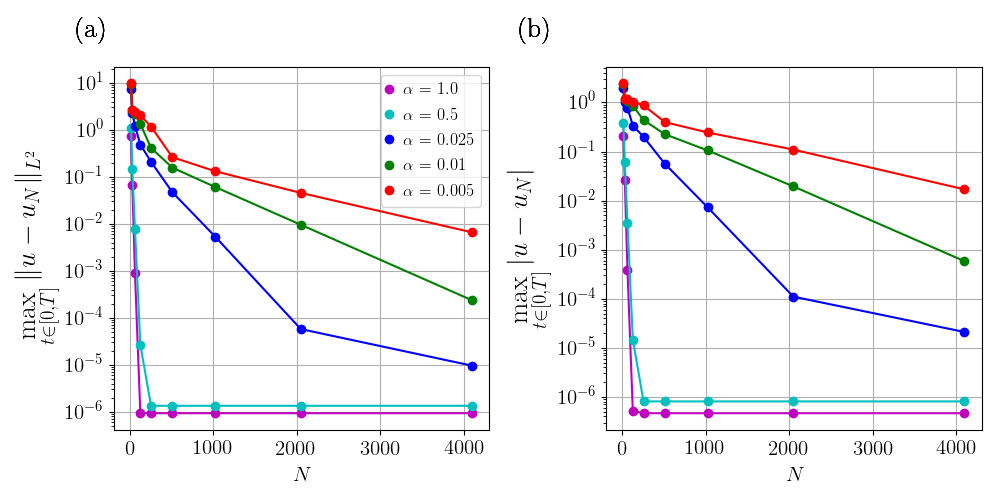
\includegraphics[width=\textwidth]{Figures/Galerkin/Graphics/alphas_Error_N.png}
    	\caption{Exact solution for (\ref{1.4}) with initial condition $u_0 (x) = e^{-(2(x - 1))^2}$ using \ref{1.9} and $\epsilon = 0.1$, $\epsilon = 0.01$ respectively.}
    	\label{Exact_Solution}
    \end{figure}
    \begin{figure}
    	\includegraphics[width=\textwidth]{Figures/Galerkin/Graphics/eps=1.0/Numerical_Solution_alpha=1.png}
    	\caption{Numerical solution for (\ref{1.4}) with initial condition $u_0 (x) = e^{- 0.05 x^2}$ using \ref{1.9} and $\alpha = 1.0$}
    	\label{Exact_Solution1}
    \end{figure}
	\begin{figure}
		\includegraphics[width=\textwidth]{Figures/Galerkin/Graphics/eps=1.0/Numerical_Solution_alpha=1_T=100.png}
		\caption{Numerical solution for (\ref{1.4}) with initial condition $u_0 (x) = e^{- 0.05 x^2}$ using \ref{1.9} and $\epsilon = 0.1$ for $t = 100$.}
		\label{Exact_Solution}
	\end{figure}
	\begin{figure}
		\includegraphics[width=\textwidth]{Figures/Galerkin/Graphics/eps=0.5/Numerical_Solution_alpha=05.png}
		\caption{Numerical solution for (\ref{1.4}) with initial condition $u_0 (x) = e^{- 0.05 x^2}$ using \ref{1.9} and $\alpha = 0.5$}
		\label{Exact_Solution}
	\end{figure}
	\begin{figure}
		\includegraphics[width=\textwidth]{Figures/Galerkin/Graphics/eps=0.5/Numerical_Solution_alpha=05_T=100.png}
		\caption{Exact solution for (\ref{1.4}) with initial condition $u_0 (x) = e^{-(2(x - 1))^2}$ using \ref{1.9} and $\epsilon = 0.1$, $\epsilon = 0.01$ respectively.}
		\label{Exact_Solution}
	\end{figure}
	\begin{figure}
		\includegraphics[width=\textwidth]{Figures/Galerkin/Graphics/eps=0.025/Numerical_Solution_alpha=0025.png}
		\caption{Numerical solution for (\ref{1.4}) with initial condition $u_0 (x) = e^{- 0.05 x^2}$ using \ref{1.9} and $\alpha = 0.025$}
		\label{Exact_Solution}
	\end{figure}
	\begin{figure}
		\includegraphics[width=\textwidth]{Figures/Galerkin/Graphics/eps=0.025/Numerical_Solution_alpha=0025_T=100.png}
		\caption{Exact solution for (\ref{1.4}) with initial condition $u_0 (x) = e^{-(2(x - 1))^2}$ using \ref{1.9} and $\epsilon = 0.1$, $\epsilon = 0.01$ respectively.}
		\label{Exact_Solution}
	\end{figure}
	\begin{figure}
		\includegraphics[width=\textwidth]{Figures/Galerkin/Graphics/eps=0.01/Numerical_Solution_alpha=001.png}
		\caption{Numerical solution for (\ref{1.4}) with initial condition $u_0 (x) = e^{- 0.05 x^2}$ using \ref{1.9} and $\alpha = 0.01$}
		\label{Exact_Solution}
	\end{figure}
	\begin{figure}
		\includegraphics[width=\textwidth]{Figures/Galerkin/Graphics/eps=0.01/Numerical_Solution_alpha=001_T=100.png}
		\caption{Exact solution for (\ref{1.4}) with initial condition $u_0 (x) = e^{-(2(x - 1))^2}$ using \ref{1.9} and $\epsilon = 0.1$, $\epsilon = 0.01$ respectively.}
		\label{Exact_Solution}
	\end{figure}
	\begin{figure}
		\includegraphics[width=\textwidth]{Figures/Galerkin/Graphics/eps=0.005/Numerical_Solution_alpha=0005.png}
		\caption{Numerical solution for (\ref{1.4}) with initial condition $u_0 (x) = e^{- 0.05 x^2}$ using \ref{1.9} and $\alpha = 0.005$}
		\label{Exact_Solution}
	\end{figure}
	\begin{figure}
		\includegraphics[width=\textwidth]{Figures/Galerkin/Graphics/eps=0.005/Numerical_Solution_alpha=0005_T=100.png}
		\caption{Exact solution for (\ref{1.4}) with initial condition $u_0 (x) = e^{-(2(x - 1))^2}$ using \ref{1.9} and $\epsilon = 0.1$, $\epsilon = 0.01$ respectively.}
		\label{Exact_Solution}
	\end{figure}
%L2
	\begin{table}
	\begin{tabular}{lcccc}
		\toprule
		\multicolumn{1}{c}{\textbf{Approximation}} & \multicolumn{4}{c}{\textbf{Error}} \\
		$\hspace{9mm}N$ & $\Delta t=1\times 10^{-2}$ & $\Delta t=1\times 10^{-3}$ & $\Delta t=1\times 10^{-4}$ & $\Delta t=1\times 10^{-5}$ \\
		\midrule
		\hspace{7mm} 16 & 0.72504    & 0.72504    & 0.72504    & 0.72504    \\
		\midrule
		\hspace{7mm} 32 & 6.90249 $\times 10 ^{-2}$   & 6.88052 $\times 10 ^{-2}$   & 6.87838 $\times 10 ^{-2}$   & 6.87816 $\times 10 ^{-2}$   \\
		\midrule
		\hspace{7mm} 64 & 1.23827 $\times 10 ^{-3}$  & 8.85367 $\times 10 ^{-4}$ & 8.80521 $\times 10 ^{-4}$ & 8.80410 $\times 10 ^{-4}$  \\
		\midrule
		\hspace{7mm} 128 & 9.43454 $\times 10 ^{-4}$ & 9.41793 $\times 10 ^{-5}$ & 9.41148 $\times 10 ^{-6}$ & 9.41827 $\times 10 ^{-7}$  \\
		\midrule
		\hspace{7mm} 256 & 9.43454 $\times 10 ^{-4}$ & 9.41793 $\times 10 ^{-5}$ & 9.41109 $\times 10 ^{-6}$ & 9.36411 $\times 10 ^{-7}$ \\
		\midrule
		\hspace{7mm} 512 & 9.43454 $\times 10 ^{-4}$ & 9.41793 $\times 10 ^{-5}$ & 9.41109 $\times 10 ^{-6}$ & 9.36411 $\times 10 ^{-7}$ \\
		\midrule
		\hspace{7mm} 1024 & $\ast$ & 9.41793 $\times 10^{-5}$ & 9.41109 $\times 10^{-6}$ & 9.36411 $\times 10^{-7}$              \\
		\midrule
		\hspace{7mm} 2048 & $\ast$ & $\ast$ & 9.41109 $\times 10^{-6}$ & 9.36411 $\times 10^{-7}$   \\
		\\
		\bottomrule
	\end{tabular}
	\caption{alpha=1.0}
	\end{table}

	\begin{table}
		\begin{tabular}{lcccc}
		\toprule
		\multicolumn{1}{c}{\textbf{Approximation}} & \multicolumn{4}{c}{\textbf{Error}} \\
		$\hspace{9mm}N$ & $\Delta t=1\times 10^{-2}$ & $\Delta t=1\times 10^{-3}$ & $\Delta t=1\times 10^{-4}$ & $\Delta t=1\times 10^{-5}$ \\
		\midrule
		\hspace{7mm} 16 & 1.08768    & 1.08714     & 1.08709     & 1.08708     \\
		\midrule
		\hspace{7mm} 32 & 0.148971   & 0.148641    & 0.148608    & 0.148605    \\
		\midrule
		\hspace{7mm} 64 & 8.08693 $\times 10^{-3}$ & 7.88502 $\times 10^{-3}$  & 7.87473 $\times 10^{-3}$  & 7.87380 $\times 10^{-3}$   \\
		\midrule
		\hspace{7mm} 128 & 1.34597 $\times 10^{-3}$ & 1.36953 $\times 10^{-4}$ & 3.01642 $\times 10^{-5}$ & 2.70428 $\times 10^{-5}$ \\
		\midrule
		\hspace{7mm} 256 & 1.34581 $\times 10^{-3}$ & 1.34281 $\times 10^{-4}$ & 1.34284 $\times 10^{-5}$ & 1.34698 $\times 10^{-6}$ \\
		\midrule
		\hspace{7mm} 512 & 1.34581 $\times 10^{-3}$ & 1.34281 $\times 10^{-4}$ & 1.34284 $\times 10^{-5}$ & 1.34698 $\times 10^{-6}$ \\
		\midrule
		\hspace{7mm} 1024 & *          & 1.34281 $\times 10^{-4}$ & 1.34284 $\times 10^{-5}$ & 1.34698 $\times 10^{-6}$ \\
		\midrule
		\hspace{7mm} 2048 & *          & 1.34281 $\times 10^{-4}$ & 1.34284 $\times 10^{-5}$ & 1.34698 $\times 10^{-6}$ \\
		\\
		\bottomrule
		\end{tabular}
		\caption{alpha=0.5}
	\end{table}	

\begin{table}
	\begin{tabular}{lcccc}
		\toprule
		\multicolumn{1}{c}{\textbf{Approximation}} & \multicolumn{4}{c}{\textbf{Error}} \\
		$\hspace{9mm}N$ & $\Delta t=1\times 10^{-2}$ & $\Delta t=1\times 10^{-3}$ & $\Delta t=1\times 10^{-4}$ & $\Delta t=1\times 10^{-5}$ \\
		\midrule
		\hspace{7mm} 16 & 7.58773    & 7.56649     & 7.56438     & 7.56417     \\
		\midrule
		\hspace{7mm} 32 & 2.26675    & 2.24916     & 2.24733     & 2.24714     \\
		\midrule
		\hspace{7mm} 64 & 1.27102    & 1.23726     & 1.23368     & 1.23332     \\
		\midrule
		\hspace{7mm} 128 & 0.498447   & 0.487193    & 0.486105    & 0.485997    \\
		\midrule
		\hspace{7mm} 256 & 0.219212   & 0.210213    & 0.209353    & 0.209267    \\
		\midrule
		\hspace{7mm} 512 & 5.2540 $\times 10^{-2}$   & 4.74419 $\times 10^{-2}$  & 4.70015 $\times 10^{-2}$  & 4.69581  $\times 10^{-2}$   \\
		\midrule
		\hspace{7mm} 1024 & 1.01652  $\times 10^{-2}$  & 5.53894 $\times 10^{-3}$  & 5.36585 $\times 10^{-3}$  & 5.35305  $\times 10^{-3}$  \\
		\midrule
		\hspace{7mm} 2048 & 9.85022 $\times 10^{-3}$ & 9.62488  $\times 10^{-4}$ & 9.60671 $\times 10^{-5}$ & 5.77595 $\times 10^{-5}$ \\
		\midrule
		\hspace{7mm} 4096 & * & 9.62487 $\times 10^{-4}$ & 9.60536 $\times 10^{-5}$ & 9.62657 $\times 10^{-6}$ \\
		\\
		\bottomrule
	\end{tabular}
	\caption{alpha=0.025}
\end{table}

\begin{table}
\begin{tabular}{lcccc}
	\toprule
	\multicolumn{1}{c}{\textbf{Approximation}} & \multicolumn{4}{c}{\textbf{Error}} \\
	$\hspace{9mm}N$ & $\Delta t=1\times 10^{-2}$ & $\Delta t=1\times 10^{-3}$ & $\Delta t=1\times 10^{-4}$ & $\Delta t=1\times 10^{-5}$ \\
	\midrule
	\hspace{7mm} 16 & 9.49461   & 9.46535    & 9.46244     & 9.46215     \\
	\midrule
	\hspace{7mm} 32 & 2.61108   & 2.59379    & 2.59219     & 2.59203     \\
	\midrule
	\hspace{7mm} 64 & 2.21422   & 2.17624    & 2.17212     & 2.17169     \\
	\midrule
	\hspace{7mm} 128 & 1.44279   & 1.35286    & 1.3432      & 1.34218     \\
	\midrule
	\hspace{7mm} 256 & 0.439921  & 0.414415   & 0.412089    & 0.411859    \\
	\midrule
	\hspace{7mm} 512 & 0.178257  & 0.158497   & 0.15711     & 0.156976    \\
	\midrule
	\hspace{7mm} 1024 & 7.19451 $\times 10^{-2}$ & 6.17976 $\times 10^{-2}$  & 6.09334 $\times 10^{-2}$   & 6.08485 $\times 10^{-2}$   \\
	\midrule
	\hspace{7mm} 2048 & 1.79845 $\times 10^{-2}$ & 1.00192 $\times 10^{-2}$  & 9.61386 $\times 10^{-3}$  & 9.57915 $\times 10^{-3}$  \\
	\midrule
	\hspace{7mm} 4096 & 1.67655 $\times 10^{-2}$ & 1.59277 $\times 10^{-3}$ & 2.62833 $\times 10^{-4}$ & 2.37279 $\times 10^{-4}$ \\
	\\
	\bottomrule
\end{tabular}
\caption{alpha=0.01}
\end{table}

\begin{table}
	\begin{tabular}{lcccc}
		\toprule
		\multicolumn{1}{c}{\textbf{Approximation}} & \multicolumn{4}{c}{\textbf{Error}} \\
		$\hspace{9mm}N$ & $\Delta t=1\times 10^{-2}$ & $\Delta t=1\times 10^{-3}$ & $\Delta t=1\times 10^{-4}$ & $\Delta t=1\times 10^{-5}$ \\
		\midrule
		\hspace{7mm} 16 & 9.95328   & 9.91901    & 9.91597    & 9.91567    \\
		\midrule
		\hspace{7mm} 32 & 2.72607   & 2.70558    & 2.70347    & 2.70326    \\
		\midrule
		\hspace{7mm} 64 & 2.50343   & 2.45988    & 2.45543    & 2.45497    \\
		\midrule
		\hspace{7mm} 128 & 2.16142   & 2.06992    & 2.05918    & 2.05795    \\
		\midrule
		\hspace{7mm} 256 & 1.3658    & 1.19385    & 1.17602    & 1.17412    \\
		\midrule
		\hspace{7mm} 512 & 0.339826  & 0.265843   & 0.262164   & 0.261805   \\
		\midrule
		\hspace{7mm} 1024 & 0.161405  & 0.133743   & 0.131882   & 0.131699   \\
		\midrule
		\hspace{7mm} 2048 & 6.50292 $\times 10^{-2}$ & 4.70602 $\times 10^{-2}$ & 4.57371 $\times 10^{-2}$  & 4.56090 $\times 10^{-2}$  \\
		\midrule
		\hspace{7mm} 4096 & * & 7.26917 $\times 10^{-3}$ & 6.64157 $\times 10^{-3}$ & 6.60753 $\times 10^{-3}$ \\
		\\
		\bottomrule
	\end{tabular}
	\caption{alpha=0.005}
\end{table}
%Max
	\begin{table}
	\begin{tabular}{lcccc}
		\toprule
		\multicolumn{1}{c}{\textbf{Approximation Max}} & \multicolumn{4}{c}{\textbf{Error}} \\
		$\hspace{9mm}N$ & $\Delta t=1\times 10^{-2}$ & $\Delta t=1\times 10^{-3}$ & $\Delta t=1\times 10^{-4}$ & $\Delta t=1\times 10^{-5}$ \\
		\midrule
		\hspace{7mm} 16 & 0.203363    & 0.203333    & 0.203331    & 0.20333     \\
		\midrule
		\hspace{7mm} 32 & 2.64192 $\times 10 ^{-2}$   & 2.6248 $\times 10 ^{-2}$    & 2.62491 $\times 10 ^{-2}$  & 2.62492 $\times 10 ^{-2}$   \\
		\midrule
		\hspace{7mm} 64 & 6.93001 $\times 10 ^{-4}$ & 4.11641 $\times 10 ^{-4}$ & 3.85563 $\times 10 ^{-4}$ & 3.82972 $\times 10 ^{-4}$ \\
		\midrule
		\hspace{7mm} 128 & 4.74934 $\times 10 ^{-4}$ & 4.73649 $\times 10 ^{-5}$ & 4.74295 $\times 10 ^{-6}$ & 5.16105 $\times 10 ^{-7}$ \\
		\midrule
		\hspace{7mm} 256 & 4.74936 $\times 10 ^{-4}$ & 4.7368 $\times 10 ^{-5}$  & 4.72569 $\times 10 ^{-6}$ & 4.64922 $\times 10 ^{-7}$ \\
		\midrule
		\hspace{7mm} 512 & 4.74936 $\times 10 ^{-4}$ & 4.7368 $\times 10 ^{-5}$  & 4.72569 $\times 10 ^{-6}$ & 4.64922 $\times 10 ^{-4}$ \\
		\midrule
		\hspace{7mm} 1024 & * & 4.7368 $\times 10 ^{-5}$  & 4.72569 $\times 10 ^{-6}$ & 4.64922 $\times 10 ^{-7}$ \\
		\midrule
		\hspace{7mm} 2048 & * & * & 4.72569 $\times 10 ^{-6}$ & 4.64922 $\times 10 ^{-7}$ \\
		\\
		\bottomrule
	\end{tabular}
	\caption{alpha=1.0}
\end{table}


\begin{table}
	\begin{tabular}{lcccc}
		\toprule
		\multicolumn{1}{c}{\textbf{Approximation Max}} & \multicolumn{4}{c}{\textbf{Error}} \\
		$\hspace{9mm}N$ & $\Delta t=1\times 10^{-2}$ & $\Delta t=1\times 10^{-3}$ & $\Delta t=1\times 10^{-4}$ & $\Delta t=1\times 10^{-5}$ \\
		\midrule
		\hspace{7mm} 16 & 0.37312     & 0.372971    & 0.372956    & 0.372954    \\
		\midrule
		\hspace{7mm} 32 & 6.02497 $\times 10 ^{-2}$   & 6.00446 $\times 10 ^{-2}$   & 6.00242 $\times 10 ^{-2}$  & 6.00221 $\times 10 ^{-2}$  \\
		\midrule
		\hspace{7mm} 64 & 4.24308 $\times 10 ^{-3}$  & 3.62765 $\times 10 ^{-3}$  & 3.56692 $\times 10 ^{-3}$ & 3.56085 $\times 10 ^{-3}$  \\
		\midrule
		\hspace{7mm} 128 & 8.17452 $\times 10 ^{-4}$ & 9.36316 $\times 10 ^{-5}$ & 2.17737 $\times 10 ^{-5}$ & 1.47495 $\times 10 ^{-5}$ \\
		\midrule
		\hspace{7mm} 256 & 8.03703 $\times 10 ^{-4}$ & 8.01354 $\times 10 ^{-5}$ & 8.01576 $\times 10 ^{-6}$ & 8.08632 $\times 10 ^{-7}$ \\
		\midrule
		\hspace{7mm} 512 & 8.03703 $\times 10 ^{-4}$ & 8.01355 $\times 10 ^{-5}$ & 8.01585 $\times 10 ^{-6}$ & 8.08658 $\times 10 ^{-7}$ \\
		\midrule
		\hspace{7mm} 1024 & * & 8.01355 $\times 10 ^{-5}$ & 8.01585 $\times 10 ^{-6}$ & 8.08658 $\times 10 ^{-7}$ \\
		\midrule
		\hspace{7mm} 2048 & * & 8.01355 $\times 10 ^{-5}$ & 8.01585 $\times 10 ^{-6}$ & 8.08658 $\times 10 ^{-7}$ \\
		\\
		\bottomrule
	\end{tabular}
	\caption{alpha=0.5}
\end{table}	

\begin{table}
	\begin{tabular}{lcccc}
		\toprule
		\multicolumn{1}{c}{\textbf{Approximation Max}} & \multicolumn{4}{c}{\textbf{Error}} \\
		$\hspace{9mm}N$ & $\Delta t=1\times 10^{-2}$ & $\Delta t=1\times 10^{-3}$ & $\Delta t=1\times 10^{-4}$ & $\Delta t=1\times 10^{-5}$ \\
		\midrule
		\hspace{7mm} 16 & 1.97657   & 1.9728     & 1.97242     & 1.97238     \\
		\midrule
		\hspace{7mm} 32 & 1.03493   & 1.02776    & 1.02703     & 1.02696     \\
		\midrule
		\hspace{7mm} 64 & 0.801199  & 0.785464   & 0.783712    & 0.783535    \\
		\midrule
		\hspace{7mm} 128 & 0.336216  & 0.338981   & 0.339247    & 0.339273    \\
		\midrule
		\hspace{7mm} 256 & 0.193548  & 0.198972   & 0.199503    & 0.199556    \\
		\midrule
		\hspace{7mm} 512 & 5.72850 $\times 10 ^{-2}$  & 5.55545 $\times 10 ^{-2}$  & 5.59961 $\times 10 ^{-2}$   & 5.6040 $\times 10 ^{-2}$     \\
		\midrule
		\hspace{7mm} 1024 & 2.33612 $\times 10 ^{-2}$ & 7.98112 $\times 10 ^{-3}$ & 7.18842 $\times 10 ^{-3}$  & 7.27570 $\times 10 ^{-3}$   \\
		\midrule
		\hspace{7mm} 2048 & 2.1658 $\times 10 ^{-2}$  & 2.12761 $\times 10 ^{-3}$ & 2.87593 $\times 10 ^{-4}$ & 1.10426 $\times 10 ^{-4}$ \\
		\midrule
		\hspace{7mm} 4096 & * & 2.10565 $\times 10 ^{-3}$ & 2.10097 $\times 10 ^{-4}$ & 2.10309 $\times 10 ^{-5}$ \\
		\\
		\bottomrule
	\end{tabular}
	\caption{alpha=0.025}
\end{table}

\begin{table}
	\begin{tabular}{lcccc}
		\toprule
		\multicolumn{1}{c}{\textbf{Approximation Max}} & \multicolumn{4}{c}{\textbf{Error}} \\
		$\hspace{9mm}N$ & $\Delta t=1\times 10^{-2}$ & $\Delta t=1\times 10^{-3}$ & $\Delta t=1\times 10^{-4}$ & $\Delta t=1\times 10^{-5}$ \\
		\midrule
		\hspace{7mm} 16 & 2.39661   & 2.38706    & 2.38611     & 2.38601     \\
		\midrule
		\hspace{7mm} 32 & 1.16756   & 1.16044    & 1.15971     & 1.15964     \\
		\midrule
		\hspace{7mm} 64 & 1.09762   & 1.06803    & 1.06597     & 1.06576     \\
		\midrule
		\hspace{7mm} 128 & 0.884737  & 0.867091   & 0.863977    & 0.863649    \\
		\midrule
		\hspace{7mm} 256 & 0.575861  & 0.449212   & 0.438762    & 0.437752    \\
		\midrule
		\hspace{7mm} 512 & 0.224554  & 0.225146   & 0.22519     & 0.225194    \\
		\midrule
		\hspace{7mm} 1024 & 0.10799   & 0.103941   & 0.105018    & 0.105126    \\
		\midrule
		\hspace{7mm} 2048 & 5.52899 $\times 10 ^{-2}$ & 2.12237 $\times 10 ^{-2}$ & 1.90972 $\times 10 ^{-2}$  & 1.94878 $\times 10 ^{-2}$   \\
		\midrule
		\hspace{7mm} 4096 & 5.75187 $\times 10 ^{-2}$ & 5.50704 $\times 10 ^{-3}$ & 9.16436 $\times 10 ^{-4}$ & 5.83005 $\times 10 ^{-4}$ \\
		\\
		\bottomrule
	\end{tabular}
	\caption{alpha=0.01}
\end{table}

\begin{table}
	\begin{tabular}{lcccc}
		\toprule
		\multicolumn{1}{c}{\textbf{Approximation Max}} & \multicolumn{4}{c}{\textbf{Error}} \\
		$\hspace{9mm}N$ & $\Delta t=1\times 10^{-2}$ & $\Delta t=1\times 10^{-3}$ & $\Delta t=1\times 10^{-4}$ & $\Delta t=1\times 10^{-5}$ \\
		\midrule
		\hspace{7mm} 16 & 2.50002  & 2.48992   & 2.48891   & 2.48881   \\
		\midrule
		\hspace{7mm} 32 & 1.21263  & 1.20544   & 1.2047    & 1.20463   \\
		\midrule
		\hspace{7mm} 64 & 1.21269  & 1.17736   & 1.17517   & 1.17495   \\
		\midrule
		\hspace{7mm} 128 & 1.10164  & 1.03493   & 1.03093   & 1.03048   \\
		\midrule
		\hspace{7mm} 256 & 0.954369 & 0.881472  & 0.873392  & 0.87259   \\
		\midrule
		\hspace{7mm} 512 & 0.665071 & 0.418735  & 0.398664  & 0.396931  \\
		\midrule
		\hspace{7mm} 1024 & 0.241841 & 0.244188  & 0.244437  & 0.244461  \\
		\midrule
		\hspace{7mm} 2048 & 0.133067 & 0.104675  & 0.109151  & 0.109596  \\
		\midrule
		\hspace{7mm} 4096 & * & 2.37273  $\times 10 ^{-2}$ & 1.75687  $\times 10 ^{-2}$ & 1.69531  $\times 10 ^{-2}$\\
		\\
		\bottomrule
	\end{tabular}
	\caption{alpha=0.005}
\end{table}

\section{Collocation Simulations}
	\begin{figure}
		\includegraphics[width=\textwidth]{Figures/Collocation/Graphics/eps=1.0/Numerical_Solution_alpha=1.png}
		\caption{Numerical solution for (\ref{1.4}) with initial condition $u_0 (x) = e^{- 0.05 x^2}$ using \ref{1.9} and $\alpha = 1.0$}
		\label{Exact_Solution1}
	\end{figure}
	\begin{figure}
		\includegraphics[width=\textwidth]{Figures/Collocation/Graphics/eps=1.0/Numerical_Solution_alpha=1_T=100.png}
		\caption{Numerical solution for (\ref{1.4}) with initial condition $u_0 (x) = e^{- 0.05 x^2}$ using \ref{1.9} and $\epsilon = 0.1$ for $t = 100$.}
		\label{Exact_Solution}
	\end{figure}
	\begin{figure}
		\includegraphics[width=\textwidth]{Figures/Collocation/Graphics/eps=0.5/Numerical_Solution_alpha=05.png}
		\caption{Numerical solution for (\ref{1.4}) with initial condition $u_0 (x) = e^{- 0.05 x^2}$ using \ref{1.9} and $\alpha = 0.5$}
		\label{Exact_Solution}
	\end{figure}
	\begin{figure}
		\includegraphics[width=\textwidth]{Figures/Collocation/Graphics/eps=0.5/Numerical_Solution_alpha=05_T=100.png}
		\caption{Exact solution for (\ref{1.4}) with initial condition $u_0 (x) = e^{-(2(x - 1))^2}$ using \ref{1.9} and $\epsilon = 0.1$, $\epsilon = 0.01$ respectively.}
		\label{Exact_Solution}
	\end{figure}
	\begin{figure}
		\includegraphics[width=\textwidth]{Figures/Collocation/Graphics/eps=0.025/Numerical_Solution_alpha=0025.png}
		\caption{Numerical solution for (\ref{1.4}) with initial condition $u_0 (x) = e^{- 0.05 x^2}$ using \ref{1.9} and $\alpha = 0.025$}
		\label{Exact_Solution}
	\end{figure}
	\begin{figure}
		\includegraphics[width=\textwidth]{Figures/Collocation/Graphics/eps=0.025/Numerical_Solution_alpha=0025_T=100.png}
		\caption{Exact solution for (\ref{1.4}) with initial condition $u_0 (x) = e^{-(2(x - 1))^2}$ using \ref{1.9} and $\epsilon = 0.1$, $\epsilon = 0.01$ respectively.}
		\label{Exact_Solution}
	\end{figure}
	\begin{figure}
		\includegraphics[width=\textwidth]{Figures/Collocation/Graphics/eps=0.01/Numerical_Solution_alpha=001.png}
		\caption{Numerical solution for (\ref{1.4}) with initial condition $u_0 (x) = e^{- 0.05 x^2}$ using \ref{1.9} and $\alpha = 0.01$}
		\label{Exact_Solution}
	\end{figure}
	\begin{figure}
		\includegraphics[width=\textwidth]{Figures/Collocation/Graphics/eps=0.01/Numerical_Solution_alpha=001_T=100.png}
		\caption{Exact solution for (\ref{1.4}) with initial condition $u_0 (x) = e^{-(2(x - 1))^2}$ using \ref{1.9} and $\epsilon = 0.1$, $\epsilon = 0.01$ respectively.}
		\label{Exact_Solution}
	\end{figure}
	\begin{figure}
		\includegraphics[width=\textwidth]{Figures/Collocation/Graphics/eps=0.005/Numerical_Solution_alpha=0005.png}
		\caption{Numerical solution for (\ref{1.4}) with initial condition $u_0 (x) = e^{- 0.05 x^2}$ using \ref{1.9} and $\alpha = 0.005$}
		\label{Exact_Solution}
	\end{figure}
	\begin{figure}
		\includegraphics[width=\textwidth]{Figures/Collocation/Graphics/eps=0.005/Numerical_Solution_alpha=0005_T=100.png}
		\caption{Exact solution for (\ref{1.4}) with initial condition $u_0 (x) = e^{-(2(x - 1))^2}$ using \ref{1.9} and $\epsilon = 0.1$, $\epsilon = 0.01$ respectively.}
		\label{Exact_Solution}
	\end{figure}
	%L2
	\begin{table}
		\begin{tabular}{lcccc}
			\toprule
			\multicolumn{1}{c}{\textbf{Approximation}} & \multicolumn{4}{c}{\textbf{Error}} \\
			$\hspace{9mm}N$ & $\Delta t=1\times 10^{-2}$ & $\Delta t=1\times 10^{-3}$ & $\Delta t=1\times 10^{-4}$ & $\Delta t=1\times 10^{-5}$ \\
			\midrule
			\hspace{7mm} 16 & 0.721112    & 0.721112    & 0.721112    & 0.721112    \\
			\midrule
			\hspace{7mm} 32 & 4.71797 $\times 10^{-2}$   & 4.72892 $\times 10^{-2}$   & 4.73004 $\times 10^{-2}$   & 4.73015 $\times 10^{-2}$   \\
			\midrule
			\hspace{7mm} 64 & 1.17954 $\times 10^{-3}$  & 7.35344 $\times 10^{-4}$ & 7.27561 $\times 10^{-4}$ & 7.27283 $\times 10^{-4}$  \\
			\midrule
			\hspace{7mm} 128 & 9.43454 $\times 10^{-4}$ & 1.75152 $\times 10^{-4}$ & 1.74583 $\times 10^{-4}$ & 1.74574 $\times 10^{-4}$ \\
			\midrule
			\hspace{7mm} 256 & 9.43454 $\times 10^{-4}$ & 1.15509 $\times 10^{-4}$ & 1.14669 $\times 10^{-4}$ & 1.14659 $\times 10^{-4}$ \\
			\midrule
			\hspace{7mm} 512 & 9.43454 $\times 10^{-4}$ & 9.41793 $\times 10^{-5}$ & 7.78847 $\times 10^{-5}$ & 7.78707 $\times 10^{-5}$ \\
			\midrule
			\hspace{7mm} 1024 & 0           & 9.41793 $\times 10^{-5}$ & 5.32213 $\times 10^{-5}$ & 5.32019 $\times 10^{-5}$ \\
			\midrule
			\hspace{7mm} 2048 & 0           & 0           & 3.56779 $\times 10^{-5}$ & 3.56498 $\times 10^{-5}$ \\
			\midrule
			\hspace{7mm} 4096 & 0           & 0           & 2.24122 $\times 10^{-5}$ & 0           \\
			\\
			\bottomrule
		\end{tabular}
		\caption{alpha=1.0}
	\end{table}
	
	\begin{table}
		\begin{tabular}{lcccc}
			\toprule
			\multicolumn{1}{c}{\textbf{Approximation}} & \multicolumn{4}{c}{\textbf{Error}} \\
			$\hspace{9mm}N$ & $\Delta t=1\times 10^{-2}$ & $\Delta t=1\times 10^{-3}$ & $\Delta t=1\times 10^{-4}$ & $\Delta t=1\times 10^{-5}$ \\
			\midrule
			\hspace{7mm} 16 & 0.721112   & 0.721112    & 0.721112    & 0.721112    \\
			\midrule
			\hspace{7mm} 32 & 0.12409    & 0.123645    & 0.123601    & 0.123596    \\
			\midrule
			\hspace{7mm} 64 & 7.66654 $\times 10^{-3}$ & 7.4129 $\times 10^{-3}$   & 7.39824 $\times 10^{-3}$  & 7.39688 $\times 10^{-3}$  \\
			\midrule
			\hspace{7mm} 128 & 1.34608 $\times 10^{-3}$ & 1.36662 $\times 10^{-4}$ & 3.00334 $\times 10^{-5}$ & 2.69743 $\times 10^{-5}$ \\
			\midrule
			\hspace{7mm} 256 & 1.34581 $\times 10^{-3}$ & 1.34281 $\times 10^{-4}$ & 1.34284 $\times 10^{-5}$ & 1.34698 $\times 10^{-6}$ \\
			\midrule
			\hspace{7mm} 512 & 1.34581 $\times 10^{-3}$ & 1.34281 $\times 10^{-4}$ & 1.34284 $\times 10^{-5}$ & 1.34698 $\times 10^{-6}$ \\
			\midrule
			\hspace{7mm} 1024 & 0          & 1.34281 $\times 10^{-4}$ & 1.34284e $\times 10^{-5}$ & 1.34698 $\times 10^{-6}$ \\
			\midrule
			\hspace{7mm} 2048 & 0          & 1.34281 $\times 10^{-4}$ & 1.34284 $\times 10^{-5}$ & 1.34698 $\times 10^{-6}$ \\
			\midrule
			\hspace{7mm} 4096 & 0          & 0           & 1.34284 $\times 10^{-5}$ & 0           \\
			\\
			\bottomrule
		\end{tabular}
		\caption{alpha=0.5}
	\end{table}	

	\begin{table}
		\begin{tabular}{lcccc}
			\toprule
			\multicolumn{1}{c}{\textbf{Approximation}} & \multicolumn{4}{c}{\textbf{Error}} \\
			$\hspace{9mm}N$ & $\Delta t=1\times 10^{-2}$ & $\Delta t=1\times 10^{-3}$ & $\Delta t=1\times 10^{-4}$ & $\Delta t=1\times 10^{-5}$ \\
			\midrule
			\hspace{7mm} 16 & 1.27349    & 1.27274     & 1.27266     & 1.27265     \\
			\midrule
			\hspace{7mm} 32 & 2.17664    & 2.15753     & 2.15573     & 2.15557     \\
			\midrule
			\hspace{7mm} 64 & 1.24009    & 1.20311     & 1.19898     & 1.19857     \\
			\midrule
			\hspace{7mm} 128 & 0.498914   & 0.486729    & 0.48555     & 0.485432    \\
			\midrule
			\hspace{7mm} 256 & 0.214295   & 0.204791    & 0.203884    & 0.203793    \\
			\midrule
			\hspace{7mm} 512 & 6.18463 $\times 10^{-2}$  & 5.65947 $\times 10^{-2}$   & 5.61273 $\times 10^{-2}$   & 5.60811 $\times 10^{-2}$   \\
			\midrule
			\hspace{7mm} 1024 & 1.00113 $\times 10^{-2}$  & 5.58983 $\times 10^{-3}$  & 5.42732 $\times 10^{-3}$  & 5.4151 $\times 10^{-3}$  \\
			\midrule
			\hspace{7mm} 2048 & 9.85022 $\times 10^{-3}$ & 9.62491 $\times 10^{-4}$ & 9.6079 $\times 10^{-5}$  & 5.41418 $\times 10^{-5}$ \\
			\midrule
			\hspace{7mm} 4096 & 0          & 9.62487 $\times 10^{-4}$ & 9.60536 $\times 10^{-5}$ & 0           \\
			\\
			\bottomrule
		\end{tabular}
		\caption{alpha=0.025}
	\end{table}
	
	\begin{table}
		\begin{tabular}{lcccc}
			\toprule
			\multicolumn{1}{c}{\textbf{Approximation}} & \multicolumn{4}{c}{\textbf{Error}} \\
			$\hspace{9mm}N$ & $\Delta t=1\times 10^{-2}$ & $\Delta t=1\times 10^{-3}$ & $\Delta t=1\times 10^{-4}$ & $\Delta t=1\times 10^{-5}$ \\
			\midrule
			\hspace{7mm} 16 & 1.33287   & 1.33206    & 1.33198     & 1.33197    \\
			\midrule
			\hspace{7mm} 32 & 2.55164   & 2.53501    & 2.53321     & 2.53303    \\
			\midrule
			\hspace{7mm} 64 & 2.20505   & 2.15802    & 2.1536      & 2.15333    \\
			\midrule
			\hspace{7mm} 128 & 1.42868   & 1.33607    & 1.32654     & 1.32551    \\
			\midrule
			\hspace{7mm} 256 & 0.43133   & 0.406296   & 0.404005    & 0.403778   \\
			\midrule
			\hspace{7mm} 512 & 0.209669  & 0.191668   & 0.19004     & 0.189879   \\
			\midrule
			\hspace{7mm} 1024 & 7.60123 $\times 10^{-2}$ & 6.45415 $\times 10^{-2}$  & 6.35566 $\times 10^{-2}$   & 6.34598 $\times 10^{-2}$  \\
			\midrule
			\hspace{7mm} 2048 & 1.81598 $\times 10^{-2}$ & 9.93558 $\times 10^{-3}$ & 9.47956 $\times 10^{-3}$ & 9.43935 $\times 10^{-3}$ \\
			\midrule
			\hspace{7mm} 4096 & 1.67655 $\times 10^{-2}$ & 1.59278 $\times 10^{-3}$ & 2.76145 $\times 10^{-4}$ & 0          \\
			\\
			\bottomrule
		\end{tabular}
		\caption{alpha=0.01}
	\end{table}

	
	\begin{table}
		\begin{tabular}{lcccc}
			\toprule
			\multicolumn{1}{c}{\textbf{Approximation}} & \multicolumn{4}{c}{\textbf{Error}} \\
			$\hspace{9mm}N$ & $\Delta t=1\times 10^{-2}$ & $\Delta t=1\times 10^{-3}$ & $\Delta t=1\times 10^{-4}$ & $\Delta t=1\times 10^{-5}$ \\
			\midrule
			\hspace{7mm} 16 & 1.36189   & 1.35883    & 1.35852   & 1.35849   \\
			\midrule
			\hspace{7mm} 32 & 2.67506   & 2.65305    & 2.65078   & 2.65055   \\
			\midrule
			\hspace{7mm} 64 & 2.50365   & 2.45855    & 2.45432   & 2.45387   \\
			\midrule
			\hspace{7mm} 128 & 2.15795   & 2.0632     & 2.05589   & 2.05497   \\
			\midrule
			\hspace{7mm} 256 & 1.362     & 1.18393    & 1.16697   & 1.16532   \\
			\midrule
			\hspace{7mm} 512 & 0.350775  & 0.304595   & 0.300865  & 0.300499  \\
			\midrule
			\hspace{7mm} 1024 & 0.168462  & 0.140332   & 0.13803   & 0.137804  \\
			\midrule
			\hspace{7mm} 2048 & 6.56161 $\times 10^{-2}$ & 4.63808 $\times 10^{-2}$  & 4.49226 $\times 10^{-2}$ & 4.47813 $\times 10^{-2}$ \\
			\midrule
			\hspace{7mm} 4096 & 0         & 7.66246 $\times 10^{-3}$ & 6.9909 $\times 10^{-3}$ & 0         \\
			\\
			\bottomrule
		\end{tabular}
		\caption{alpha=0.005}
	\end{table}

	%Max
	\begin{table}
		\begin{tabular}{lcccc}
			\toprule
			\multicolumn{1}{c}{\textbf{Approximation Max}} & \multicolumn{4}{c}{\textbf{Error}} \\
			$\hspace{9mm}N$ & $\Delta t=1\times 10^{-2}$ & $\Delta t=1\times 10^{-3}$ & $\Delta t=1\times 10^{-4}$ & $\Delta t=1\times 10^{-5}$ \\
			\midrule
			\hspace{7mm} 16 & 0.317617    & 0.317617    & 0.317617    & 0.317617    \\
			\midrule
			\hspace{7mm} 32 & 1.95279 $\times 10 ^{-2}$  & 1.96812 $\times 10 ^{-2}$   & 1.96965 $\times 10 ^{-2}$   & 1.96981 $\times 10 ^{-2}$   \\
			\midrule
			\hspace{7mm} 64 & 6.21793 $\times 10 ^{-4}$ & 2.9813 $\times 10 ^{-4}$  & 2.80086 $\times 10 ^{-4}$ & 2.78934 $\times 10 ^{-4}$ \\
			\midrule
			\hspace{7mm} 128 & 4.74952 $\times 10 ^{-4}$ & 1.64746 $\times 10 ^{-4}$ & 1.6473 $\times 10 ^{-4}$  & 1.64728 $\times 10 ^{-4}$ \\
			\midrule
			\hspace{7mm} 256 & 4.74936 $\times 10 ^{-4}$ & 1.52482 $\times 10 ^{-4}$ & 1.52467 $\times 10 ^{-4}$ & 1.52465 $\times 10 ^{-4}$ \\
			\midrule
			\hspace{7mm} 512 & 4.74936 $\times 10 ^{-4}$ & 1.47249 $\times 10 ^{-4}$ & 1.47234 $\times 10 ^{-4}$ & 1.47232 $\times 10 ^{-4}$ \\
			\midrule
			\hspace{7mm} 1024 & 0           & 1.45032 $\times 10 ^{-4}$ & 1.45017 $\times 10 ^{-4}$ & 1.45016 $\times 10 ^{-4}$ \\
			\midrule
			\hspace{7mm} 2048 & 0           & 0           & 1.43941 $\times 10 ^{-4}$ & 1.4394 $\times 10 ^{-4}$ \\
			\midrule
			\hspace{7mm} 4096 & 0           & 0           & 1.43411 $\times 10 ^{-4}$ & 0           \\
			\\
			\bottomrule
		\end{tabular}
		\caption{alpha=1.0}
	\end{table}
	
	
	\begin{table}
		\begin{tabular}{lcccc}
			\toprule
			\multicolumn{1}{c}{\textbf{Approximation Max}} & \multicolumn{4}{c}{\textbf{Error}} \\
			$\hspace{9mm}N$ & $\Delta t=1\times 10^{-2}$ & $\Delta t=1\times 10^{-3}$ & $\Delta t=1\times 10^{-4}$ & $\Delta t=1\times 10^{-5}$ \\
			\midrule
			\hspace{7mm} 16 & 0.317617    & 0.317617    & 0.317617    & 0.317617    \\
			\midrule
			\hspace{7mm} 32 & 5.04627 $\times 10 ^{-2}$   & 5.01587 $\times 10 ^{-2}$ $\times 10 ^{-2}$  & 5.01284 $\times 10 ^{-2}$  & 5.01254 $\times 10 ^{-2}$   \\
			\midrule
			\hspace{7mm} 64 & 3.72706 $\times 10 ^{-3}$  & 3.12999 $\times 10 ^{-3}$  & 3.07095 $\times 10 ^{-3}$ & 3.06507 $\times 10 ^{-3}$  \\
			\midrule
			\hspace{7mm} 128 & 8.12297 $\times 10 ^{-4}$ & 9.1143 $\times 10 ^{-5}$  & 2.01844 $\times 10 ^{-5}$ & 1.31125 $\times 10 ^{-5}$ \\
			\midrule
			\hspace{7mm} 256 & 8.03703 $\times 10 ^{-4}$ & 8.01354 $\times 10 ^{-5}$ & 8.0158 $\times 10 ^{-6}$  & 8.08554 $\times 10 ^{-7}$ \\
			\midrule
			\hspace{7mm} 512 & 8.03703 $\times 10 ^{-4}$ & 8.01355 $\times 10 ^{-5}$ & 8.01585 $\times 10 ^{-6}$ & 8.08658 $\times 10 ^{-7}$ \\
			\midrule
			\hspace{7mm} 1024 & * & 8.01355 $\times 10 ^{-5}$ & 8.01585 $\times 10 ^{-6}$ & 8.08658 $\times 10 ^{-7}$ \\
			\midrule
			\hspace{7mm} 2048 & * & 8.01355 $\times 10 ^{-5}$ & 8.01585 $\times 10 ^{-6}$ & 8.08658 $\times 10 ^{-7}$ \\
			\midrule
			\hspace{7mm} 4096 & * & *  & 8.01585 $\times 10 ^{-6}$ & 8.08658 $\times 10 ^{-7}$ \\
			\\
			\bottomrule
		\end{tabular}
		\caption{alpha=0.5}
	\end{table}	
	
	\begin{table}
		\begin{tabular}{lcccc}
			\toprule
			\multicolumn{1}{c}{\textbf{Approximation Max}} & \multicolumn{4}{c}{\textbf{Error}} \\
			$\hspace{9mm}N$ & $\Delta t=1\times 10^{-2}$ & $\Delta t=1\times 10^{-3}$ & $\Delta t=1\times 10^{-4}$ & $\Delta t=1\times 10^{-5}$ \\
			\midrule
			\hspace{7mm} 16 & 0.641596  & 0.641482   & 0.641471    & 0.64147     \\
			\midrule
			\hspace{7mm} 32 & 1.0007    & 0.992986   & 0.992194    & 0.992115    \\
			\midrule
			\hspace{7mm} 64 & 0.792843  & 0.775879   & 0.773887    & 0.773684    \\
			\midrule
			\hspace{7mm} 128 & 0.33336   & 0.336162   & 0.336499    & 0.336532    \\
			\midrule
			\hspace{7mm} 256 & 0.194832  & 0.199762   & 0.200243    & 0.200291    \\
			\midrule
			\hspace{7mm} 512 & 7.19666 $\times 10 ^{-2}$ & 6.85241 $\times 10 ^{-2}$ & 6.94956 $\times 10 ^{-2}$  & 6.95925 $\times 10 ^{-2}$   \\
			\midrule
			\hspace{7mm} 1024 & 2.38907 $\times 10 ^{-2}$ & 9.33421 $\times 10 ^{-3}$ & 8.04173 $\times 10 ^{-3}$  & 8.00305 $\times 10 ^{-3}$  \\
			\midrule
			\hspace{7mm} 2048 & 2.15954 $\times 10 ^{-2}$ & 2.11565 $\times 10 ^{-3}$ & 2.76915 $\times 10 ^{-4}$ & 1.17508 $\times 10 ^{-4}$ \\
			\midrule
			\hspace{7mm} 4096 & 0         & 2.10565 $\times 10 ^{-3}$ & 2.10101 $\times 10 ^{-4}$ & 0           \\
			\\
			\bottomrule
		\end{tabular}
		\caption{alpha=0.025}
	\end{table}

	
	\begin{table}
		\begin{tabular}{lcccc}
			\toprule
			\multicolumn{1}{c}{\textbf{Approximation Max}} & \multicolumn{4}{c}{\textbf{Error}} \\
			$\hspace{9mm}N$ & $\Delta t=1\times 10^{-2}$ & $\Delta t=1\times 10^{-3}$ & $\Delta t=1\times 10^{-4}$ & $\Delta t=1\times 10^{-5}$ \\
			\midrule
			\hspace{7mm} 16 & 0.681076  & 0.680949   & 0.680936   & 0.680935  \\
			\midrule
			\hspace{7mm} 32 & 1.15049   & 1.14135    & 1.14041    & 1.14032   \\
			\midrule
			\hspace{7mm} 64 & 1.08584   & 1.0603     & 1.05767    & 1.05741   \\
			\midrule
			\hspace{7mm} 128 & 0.891736  & 0.860129   & 0.857171   & 0.857009  \\
			\midrule
			\hspace{7mm} 256 & 0.559369  & 0.43683    & 0.426464   & 0.425438  \\
			\midrule
			\hspace{7mm} 512 & 0.248958  & 0.256402   & 0.257123   & 0.257195  \\
			\midrule
			\hspace{7mm} 1024 & 0.11386   & 0.109425   & 0.111153   & 0.111325  \\
			\midrule
			\hspace{7mm} 2048 & 5.49393 $\times 10 ^{-2}$ & 1.97643 $\times 10 ^{-2}$  & 1.97064 $\times 10 ^{-2}$  & 1.99969 $\times 10 ^{-2}$ \\
			\midrule
			\hspace{7mm} 4096 & 5.71082 $\times 10 ^{-2}$ & 5.42883 $\times 10 ^{-3}$ & 9.5015 $\times 10 ^{-4}$ & 0         \\
			\\
			\bottomrule
		\end{tabular}
		\caption{alpha=0.01}
	\end{table}

	
	\begin{table}
		\begin{tabular}{lcccc}
			\toprule
			\multicolumn{1}{c}{\textbf{Approximation Max}} & \multicolumn{4}{c}{\textbf{Error}} \\
			$\hspace{9mm}N$ & $\Delta t=1\times 10^{-2}$ & $\Delta t=1\times 10^{-3}$ & $\Delta t=1\times 10^{-4}$ & $\Delta t=1\times 10^{-5}$ \\
			\midrule
			\hspace{7mm} 16 & 0.695784 & 0.695659  & 0.695646  & 0.695645 \\
			\midrule
			\hspace{7mm} 32 & 1.20278  & 1.19418   & 1.19329   & 1.1932   \\
			\midrule
			\hspace{7mm} 64 & 1.22454  & 1.18903   & 1.18507   & 1.18467  \\
			\midrule
			\hspace{7mm} 128 & 1.11999  & 1.0238    & 1.01754   & 1.01701  \\
			\midrule
			\hspace{7mm} 256 & 0.927954 & 0.877058  & 0.872508  & 0.87201  \\
			\midrule
			\hspace{7mm} 512 & 0.664133 & 0.415288  & 0.39714   & 0.395563 \\
			\midrule
			\hspace{7mm} 1024 & 0.247742 & 0.259451  & 0.260605  & 0.26072  \\
			\midrule
			\hspace{7mm} 2048 & 0.126824 & 0.103297  & 0.107102  & 0.10748  \\
			\midrule
			\hspace{7mm} 4096 & 0        & 2.04624 $\times 10 ^{-2}$ & 1.76513  $\times 10 ^{-2}$ & 0        \\
			\\
			\bottomrule
		\end{tabular}
		\caption{alpha=0.005}
	\end{table}

%\midrule
%300(149,4) & $0.14075$ & $1.38483 \times 10 ^{-2}$ & $1.23881 \times 10 ^{-3}$ & $1.48678 \times 10 ^{-2}$ \\
%\midrule
%150(74,4) & $0.12869$ & $1.12384 \times 10 ^{-2}$ & $1.17882 \times 10 ^{-2}$ & $0.16034$ \\
%\\

    

	